In the last three chapters, we have presented our methodology to assess the
performance evolution history of configurable software systems. The first part
covered a catalog of methods to derive a variability model from the software
system or related resources along with different strategies to select sample
sets of variants. In the second part, we presented and evaluated different
strategies to select a subset of revisions, for which performance measurements
approximate the overall performance evolution history. The third part reviewed
aspects on concrete performance measurement, including guidelines to follow when choosing
a benchmark to test, and when summarizing measurement results across different
variants and versions.

While the evaluation of revision sampling strategies in the previous chapter
already presented some performance measurement results ex ante, in this chapter, we
evaluate the applicability of our methodology with a case study. With our case
study we intend to answer the following research questions:

\begin{enumerate}[$RQ_1$)]
  \item \emph{Can we recover a performance evolution history?}
  \item \emph{Does performance evolve for configurable software systems?}
  \item \emph{What revision sampling strategies accurately sketch performance evolution history?}
  \item \emph{Following our methodology, do we obtain reliable performance
  measurements?}
\end{enumerate}

This chapter is organized as follows. In section\,\ref{sec:casestudy} we present
our case study corpus, i.e., the selection of configurable software systems that we
assess performance for in our experiment. Section\,\ref{sec:expsetup} addresses
$RQ_1$ by documenting how we followed our methodology throughout the experiment
setup and conduction. Section\,\ref{sec:expresults} addresses $RQ_2$  with an
extensive description of performance evolution results and insights obtained from it.
Finally, section\,\ref{sec:reliability} addresses $RQ_3$ and $RQ_4$ by reviewing
the accuracy of revision sampling strategies and assessing the reliability of our performance measurement approach.

\section{Case Study Corpus}\label{sec:casestudy}
To evaluate our methodology, we selected two subject systems: GNU XZ and
x264. The selection process accounted for the following requirements. First,
since our intention is to assess the performance evolution history of a
configurable software system, we limited our selection to mature software
systems that exhibit a development history of a couple years or more. Second,
we limit our selection to software systems for which we can obtain a
fine-grained development history, usually version control logs. The rationale is
that our methodology considers the sampling of different revisions as well as the possibility to manually inquire possible causes of performance
changes. Third, we intend to consider software systems that have already been
subject of related research, such as work on performance prediction models.
This enables us to compare our results with, and place our results in the
context of previous work. Lastly, the scope of this case study is constrained
by limited time. Hence, the selection of software systems to assess is not
representative, yet intended to validate the methodology presented earlier, and
to obtain empirical insights on whether, and if so, how performance evolves for
configurable software systems.

Our case study corpus comprises two configurable software systems, GNU
XZ\footnote{Find the project description of GNU XZ at
\url{https://tukaani.org/xz/}.} and x264\footnote{Find the project description
of x264 at \url{https://www.videolan.org/developers/x264.html}.}.
GNU XZ is a free file compression tool that is widely used across the open-source universe. GNU XZ provides a development history of about ten years,
or more than 1,100 versions,  and is actively maintained as part of the GNU
project. It provides a publicly accessible Git repository as well as additional
resources, such as archived mailing lists and bug reports. The software itself
has not been subject of related research, yet it has been frequently compared
with other file compression tools with respect to compression performance. 

x264 is a free library implementation of the H.264 codec for video encoding,
commonly known as MPEG-4. The implementation provides a command line interface
to use and has been subject of previous research, including performance
prediction models
\citep{siegmund_predicting_2012,siegmund_performance-influence_2015}. Similar to
GNU XZ, x264 is a mature software system that provides a development history of almost ten years, or more than 2,800 versions. Both software systems are configurable at load-time
via command line arguments that modify the file compression process, or video
encoding process, respectively.

\section{$RQ_1$: Can we recover a performance evolution history?}\label{sec:expsetup} 
In the following, we document the application of our methodology to the two
software systems of our case study corpus. In particular, this section covers
the aspects of variability- and performance assessment since we have already
covered the results for revision sampling in chapter\,\ref{chapter:4}. 

All performance measurements made in the
following were conducted on a Linux machine (Debian 8) with a Intel Xeon
E5-2680 v2 with 2.8 GHz and 16 GB RAM. For each version and variant, we
repeatedly executed  a benchmark five times and selected the median of the
resulting measurements to minimize the impact of biased measurements.

\subsection{Application of our methodology to GNU XZ}
\paragraph{Variability Assessment.} For GNU XZ, we considered the application’s
man page documentation to synthesize a variability model since we could not
find any more comprehensive documentation artifacts (cf. the use cases in
Table\,\ref{tab:synthesis} as well as the questionnaire in
Table\,\ref{tab:manual_var_assessment}).
GNU XZ is configurable at build-time via command-line arguments passed to the program with every execution. Since the application is a file compression utility, it provides two operation modes,
file compression and decompression. For our evaluation, we chose to assess
performance for file compression as most compression tools are compared by
compression performance rather than decompression. We extracted configuration
options based on two criteria from the man page documentation. First, a command
line argument is a valid configuration option if it relates to the chosen
operation mode. This specifically excludes options, such as command line
arguments to return the version number, or to affect user interaction. Second,
a command line argument is a valid configuration option if it does not alter
the configuration of other options. This especially applies to presets which on
the one hand relate to the chosen operation mode, but on the other hand
preselect values for other configuration options. While for some configuration
parameters, domains were explicitly specified, for those options remaining
unspecified we had to manually investigate minimum or maximum values by
trial-and-error. In total, we identified nine binary, four numeric
configuration options, and two constraints, resulting in $7.22 \times 10^{14}$
possible variants considering the domains of numeric configuration options.

Using pair-wise sampling (cf. Section\,\ref{sec:configuration_sam}), we selected
36 variants for which we assess their performance. We selected pair-wise sampling over the other
mentioned sampling methods as we cover all pair-wise feature interactions with
very few configurations. The feature model in terms of configuration option
parameters has not changed during the development history as the man page has
never been revised significantly. In fact, the documentation lists a number of
configuration options whose corresponding features have not been implemented
yet, for instance support for multi-threading.

\paragraph{Performance Assessment.} For GNU XZ, we selected the Canterbury
corpus (2.8 MB) as the benchmark. The Canterbury corpus is a standardized set of files that is
intended to be representative since it contains files of different types, such
as text or binary data. To measure performance of GNU XZ, we refer to the
execution time since the benchmark file as well as the implemented compression
algorithm remain unchanged for all versions and variants. We conceive any
increase in execution time as performance degradation, and any decrease in
execution time measurements as an increase in performance quality properties.
Further possible performance indicators for GNU XZ beside the execution time
include the compression ratio (ratio of uncompressed input and compressed
output), and the resource utilization. With respect to the limited scope of the
thesis, and, for the sake of comparability, we only take into account execution
time.

\subsection{Application of our methodology to x264}
\paragraph{Variability Assessment.} For x264, similar to GNU XZ, the most
comprehensive documentation, and, therefore our primary source of information for the
synthesis of a variability model was the software system’s man page. x264 is
configurable at load-time and can be configured via command-line arguments
passed when executing the program. The software provides only one operation
mode, the encoding of uncompressed video data, yet it can be tuned with a range
of command-line parameters. We only selected those parameters as configuration
options that relate to the operation mode, and excluded preset parameters. For
instance, we excluded a command-line parameter that specifies how many video
frames at the beginning of the video should be dropped. In total, we identified
eight binary options, twelve numeric options, and no constraint, resulting in
$7.98 \times 10^{23}$ variants considering the domains of numeric configuration
options.

Using pair-wise sampling (cf. Section\,\ref{sec:configuration_sam}) we selected
a sample set of eight variants for which we assess their performance. As the binary configuration
options are optional, we required very few configurations to cover all
pair-wise feature interactions.

\paragraph{Performance Assessment.} We selected an uncompressed video file (79.9
MB) provided by the Xiph.org foundation as a benchmark to encode as an MP4 file.
Similar to GNU XZ, we consider the execution time as the key performance
indicator since the benchmark file as well as the implemented encoding standard
remain unchanged for all versions and variants. We conceive any increase in
execution time as performance degradation, and any decrease in execution time
measurements as an increase in performance quality properties. Again, we could
consider additional performance indicators, such as throughput in terms of
frames encoded per second. However, with respect to the limited scope of this
thesis, and, to compare performance results across systems, we decided to only
focus on execution time.\\

All in all, the methodology provided a guideline to obtain
performance evolution results. In particular, for the synthesis of variability
models as well as the selection of suitable performance benchmarks, the
methodology provided conceptual decisions in terms of which use case to refer
to. However, the methodology remains generic rather than concrete in other
aspects, such as the recommendation of variant- or version sampling strategies.
For variant sampling, the specification of coverage criteria is left to the
practicioner, and, for version sampling, the suitability of a sampling strategy
might also depend on the shape of the overall performance evolution history
(cf. section\,\ref{sec:revsampling_method}).

\section{$RQ_2$: Does performance evolve for configurable software systems?}\label{sec:expresults}
We have evaluated the performance evolution history results regarding two
aspects, effect magnitude and effect range. For both aspects, we ask whether
there are patterns or trends. A pattern in our context is a recurring shape of
segments of an performance history curve. In addition, we define a trend as a
more global increase or decrease in performance measurements that might
superpose local patterns.

\subsection{Effect magnitude}
To investigate the magnitude of changes in performance measurements, we consider
the relative changes from commit to commit rather than the absolute changes
since most variants exhibited different levels of performance measures as some
variants performed better than others, depending on the respective
configuration~(cf. section\,\ref{sec:relativechange}). To illustrate the relative
performance changes, in Figure\,\ref{fig:relative_changes} we present the relative performance changes
of the best- and worst-performing variants along with a medium performing
variant for both systems respectively.
In addition, we provide a zero baseline (grey) to illustrate whether
performance measurements increase (curve above the baseline) or decrease
(curve below the baseline).

\paragraph{Patterns.} For both systems we can see local fluctuations in
the relative performance changes. For GNU XZ, however, the different versions
fluctuate more heterogeneously starting from commit 250. 

For this first commit 
segment as well as for x264, commits with a performance degradation have commit
messages indicating the introduction of new features to the software system. For
commits for which performance improves, commit messages suggest that program
errors have been fixed.

\paragraph{Trends.} With respect to our zero-change baseline, we can see that
for GNU XZ, the vast majority of commits result in a performance regression,
while for x264, the distribution of performance-increasing and -decreasing commits is more balanced. This indicates a global trend for  GNU
XZ, where performance has degraded over the course of ten years, while for
x264, performance, besides more local fluctuations, has not degraded
significantly.

\begin{figure}[!htb]
\def\tabularxcolumn#1{m{#1}}
\begin{tabularx}{\linewidth}{@{}cXX@{}}
\centering
\begin{tabular}{c}
\subfloat[GNU XZ]
{\includegraphics[width=1.0\textwidth]{images/xz_changes.eps}}
\\
\subfloat[x264]
{\includegraphics[width=1.0\textwidth]{images/x264_changes.eps}}
\end{tabular}
\end{tabularx}
\caption{Relative commit-to-commit change in execution time in percent for GNU
XZ and x264. Depicted are curves for three variants for both systems
respectively. The illustrated best-, medium-, and worst-performing variant
exhibited the best, average, and worst average execution time across all
versions.}
\label{fig:relative_changes}
\end{figure}

\subsection{Effect range}
To summarize the performance evolution with respect to the effect range, we ask
the question whether multiple variants change homogeneously for the same version.
Therefore, we first computed the relative performance change form commit to
commit for each variant. Second, we have computed the variance of relative
performance changes per version. The rationale behind this is that if for a new
version all variants’ performance changes homogeneously, the resulting variance
is low, whereas if variants change heterogeneously, the resulting variance is
high~(cf. section\,\ref{sec:changevar}). For both GNU XZ and x264, we present the
variance of performance changes over time in Figure\,\ref{fig:change_variance}. In addition to the smoothed
curve, we provide the global average variance to indicate global trends.

\paragraph{Patterns.} Similar to the effect magnitude, we can see local
fluctuations in the variance of performance changes for the beginning of GNU
XZ’s history as well as throughout all of x264’s history. These fluctuations
suggest that for some time, variants evolved more homogeneously, followed by a
time span where variants evolved more independently.

\paragraph{Trends.} For GNU XZ, we identified a global increase in variance
among performance changes while simultaneously, the amplitude of fluctuations
decreased. That is, variants continued evolving more heterogeneously over the
development history. Moreover, the older the software system, the fewer
versions seem to change performance of all variants. For x264, however, we
observe more fluctuations throughout all the history, indicating that from time to time
commits did affect more variants than others. In addition, the variance does
not increase on a global scope. This indicates that most variants kept evolving
homogeneously throughout the development history.

\begin{figure}[!htb]
\def\tabularxcolumn#1{m{#1}}
\begin{tabularx}{\linewidth}{@{}cXX@{}}
\centering
\begin{tabular}{c}
\subfloat[GNU XZ]
{\includegraphics[width=1.0\textwidth]{images/xz_variance.eps}}
\\
\subfloat[x264]
{\includegraphics[width=1.0\textwidth]{images/x264_variance.eps}}
\end{tabular}
\end{tabularx}
\caption{Variance of relative execution time changes across all variants of a
software system. While the markers depict values for a single version/commit,
the smoothed curve visualizes local trends. The baseline depicts the global
average variance of relative performance change.}
\label{fig:change_variance}
\end{figure}

\subsection{What can be learn from a performance history?}\label{sec:expconc}
The described performance results in the previous section suggest that both
software systems exhibit different quality attributes with respect to their
software architecture. In this last subsection, we place the observed results
in the context of existing work on software evolution mentioned in
section\,\ref{sec:evolving_solftware}.

\paragraph{GNU XZ.} For GNU XZ, based on our observations, we can say that the
software architecture in the beginning was ductile in the beginning and got more brittle
over the time since fluctuations in the performance change variance decreased;
also, the variance of performance changes increased during the development
history suggesting a more chaotic performance evolution for each variant. This
is in line with our observation in Figure\,\ref{fig:ActivityGraphs}, where the
best-performing variant changes significantly stronger compared to the other two variants. The
concept of technical debt \citep{guo_tracking_2011}, meaning a global trend of
performance degradation can be identified as well. Interestingly, GNU XZ was revised
more frequently in the beginning of the development history than more recently.
All in all, the observations suggest that GNU XZ today exhibits a poor software
architecture that has become brittle as most of the committed versions are
older than five years and very few commits did affect variants homogeneously.

\paragraph{x264.} In contrast to GNU XZ, the observations for x264 indicate that
the software architecture remained ductile during the development history for a number of
reasons. First, the fluctuations in the variance of performance changes did not
decrease significantly over time indicating that more recent commits can have
the same effect on performance as more older ones. Moreover, the overall
variance of performance change, besides the aforementioned fluctuations, did
not increase. Second, the performance measurements for x264 fluctuate, but do
not exhibit a global trend similar to GNU XZ. This shows that both the effect
magnitude as well as the effect range for performance changes remained stable
during the development history. All in all, the observations suggest that the software architecture of x264 is
more mature than GNU XZ.

\section{$RQ_3$ and $RQ_4$: Accuracy and Reliability}
\label{sec:reliability} In this final evaluation section we evaluate the
methodology with respect to accuracy ($RQ_3$) and ($RQ_4$). $RQ_3$ asks, whether
our methodology can accurately describe performance evolution for a given
configurable software system, and $RQ_4$ asks, whether the measurements we
obtain our performance evolution history from are reliable.

\paragraph{Accuracy.} With regard to the partial
evaluation of revision sampling strategies in chapter\,\ref{chapter:4}, where we
evaluated accuracy, no definitive answer can be given.
The used case study of only two configurable software systems is too small to make a reliable statement
here. However, what we have learned from the two software systems was that we
could not clearly distinguish accuracy measures for different revision sampling
strategies for x264, presumably due to a performance evolution history curve
that only exhibits small-sized fluctuations. In other words, the curve for x264
is shaped quasi-linear and therefore easily approximated by any selection of
sample points. Leaving the indecisive accuracy evaluation for x264 as well as
the size of the case study corpus aside, at least, the accuracy results for GNU
XZ suggest that the best-performing revision sampling strategies can accurately
select a sample of revisions to sketch performance evolution. Nonetheless, this
question requires further research to reliably recommend and ensure a accurate
revision sampling strategy.

\paragraph{Reliability.} To assess reliability for our methodology, we ask
whether performance measurements using our methodology are reproducible, i.e.,
if we obtain similar measurements under similar conditions. We answer
$RQ_4$ by conducting a small case study. We measure the spread of
execution time measurements to check whether spread is influenced by the
software system tested, the execution time, or the number of repetitions.
During all experiments in our evaluation, we have used five repetitions per
version and variant. This experiment is merely intended to validate the
reliability of this decision. 

\begin{wrapfigure}{r}{0.5\textwidth}
 \begin{center}
   \vspace{-1cm}
   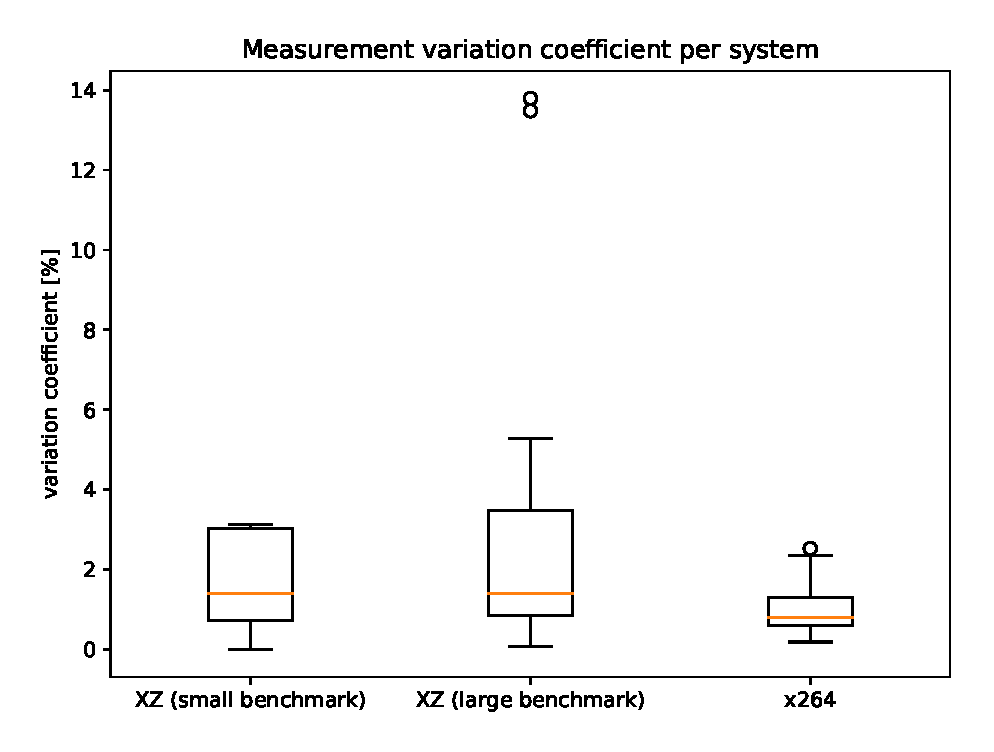
\includegraphics[width=0.48\textwidth]{images/reliability_1.eps}
 \end{center}
 \caption{Distributions of variation coefficients for
 GNU XZ (for two different benchmarks), and for x264.
 Measured median variation coefficients were
 1.408\,\% and 1.40\,\% for GNU XZ, and 0.794\,\% for
 x264.}\label{fig:reliability_1}
\end{wrapfigure}

For this experiment, of the two
sample system GNU XZ and x264, we selected three variants each. Each of the
three variants is derived from configuration presets with the incentive to
obtain a fast-,  medium-, and a slow-performing variant. The rationale behind this
approach is that conclusions about a configurable software system drawn from
multiple variants are more valid than simply measuring one arbitrary variant.
In addition, this choice allows us to investigate the influence of the
execution time on spread as we expect different levels of execution time
measurements. Each experiment was repeated three to 20 times. Finally, since
the execution time measurements for the Canterbury corpus for GNU XZ were
relatively small (around one second), we tested the same three variants with an
additional benchmark which is the Canterbury corpus tripled in size.

First, we investigated the influence of the configurable software system
studied. Therefore, in Figure\,\ref{fig:reliability_1}, we illustrate the
distribution of the variation coefficients for each experiment per system. The variation
coefficient is computed as the  standard deviation of the execution time divided
by (or normalized to) the arithmetic mean in order to compare the measures of
spread for arbitrary distributions. 
We see that for GNU XZ, regardless of the benchmark, the variation coefficient
is almost two times higher than for x264. This observation indicates, that for
GNU XZ, the execution time measurement variance is notably higher, suggesting
that the software system tested has an influence on how strongly measurements
can spread.

\begin{figure}
\centering
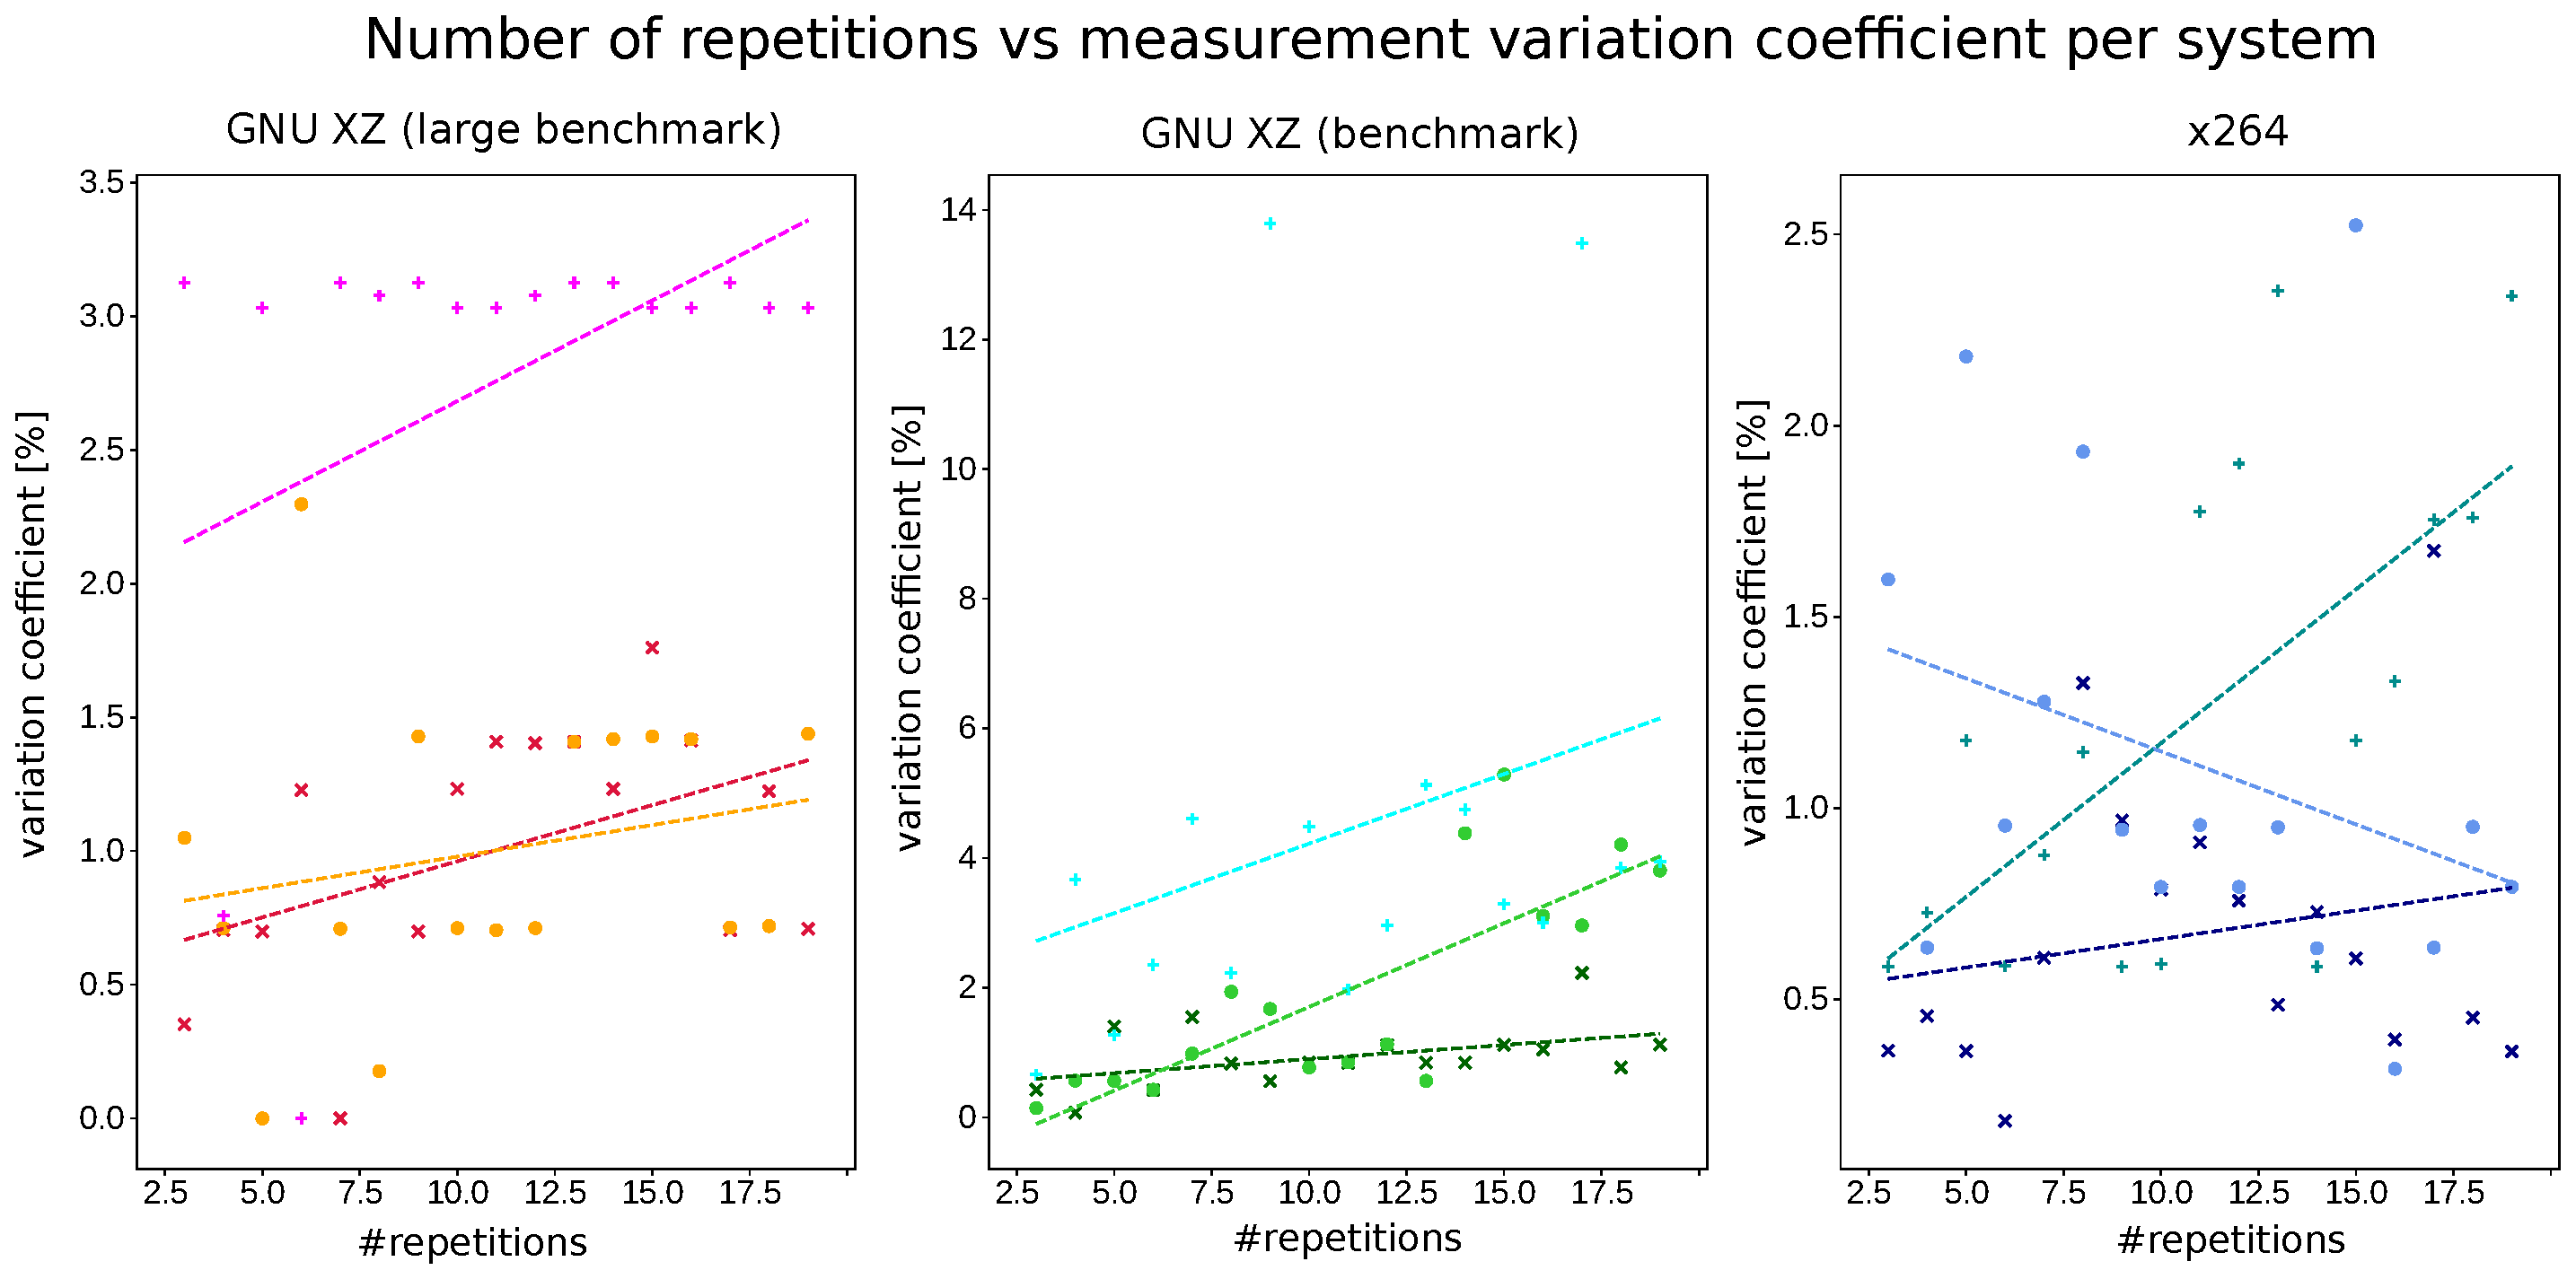
\includegraphics[width=0.99\textwidth]{images/reliability_3.eps}
\caption{Number of repetitions vs execution time measurement variation
coefficients for GNU XZ and x264. For GNU XZ, we tested two benchmarks
differing in size (the Canterbury corpus and a triple copy thereof). For each
subplot, we present three variants, one slow-, one medium-, and one
fast-performing one, each depicted by different colors and markers (\texttt{x}:
slow, \texttt{o}:medium, \texttt{+}: fast).}\label{fig:reliability_3}
\end{figure}

Second, we investigated the influence of the number of repetitions on the
variation coefficient of execution time measurements. In
Figure\,\ref{fig:reliability_3}, we illustrate the variation coefficients
plotted against the number of repetitions. We colorized each variant uniquely,
and assigned markers for each variant (\texttt{x} for the slow-,
{\texttt{o}} for the medium-, and \texttt{+} for the fast-performing variants).
In addition, we provided best linear fit curves of the same color to identify possible
trends. However, non of the presented fits suggests a significant relationship.

In conclusion, the only significant influence we could determine in our small
reliability assessment was the influence of the configurable software system
studied. The results suggest, that the software system studied influences the
reliability of execution time measurements. Further investigation, in particular
with regard to the question, what properties of a configurable software system
drive the impact on reliability, is required to determine the degree of
(non-)determinism of a configurable software system. However, this question
exceeds the scope of this thesis. All in all, we conclude that performance, or
execution time measurements using the Unix \texttt{time} command are sufficiently
reliable for the purpose of assessing the performance evolution of configurable
software systems.



